\documentclass[10pt, compress]{beamer}
\usetheme[titleprogressbar]{m}

\usepackage{booktabs}
\usepackage[scale=2]{ccicons}
\usepackage{minted}

\usepgfplotslibrary{dateplot}

\usemintedstyle{trac}

\title{The Loewner Equation and the derivative of its solution}
\subtitle{}
\author{Carl Ringqvist}
\institute{Master's Thesis presentation, KTH \& SU}

\begin{document}

\maketitle

\begin{frame}[fragile]
\frametitle{Introduction}
Charles Loewner and the introduction of the Loewner Equation.
% The future demands more efficient computing

% not achievable by common sequential programming 

% CUDA and OpenCL exists, but is a nuisance to write, and to use in mainstream languages

% we want a way to both develop and use efficient GPU computational kernels
% within mainstream language contexts.


\begin{figure}
  \centering
 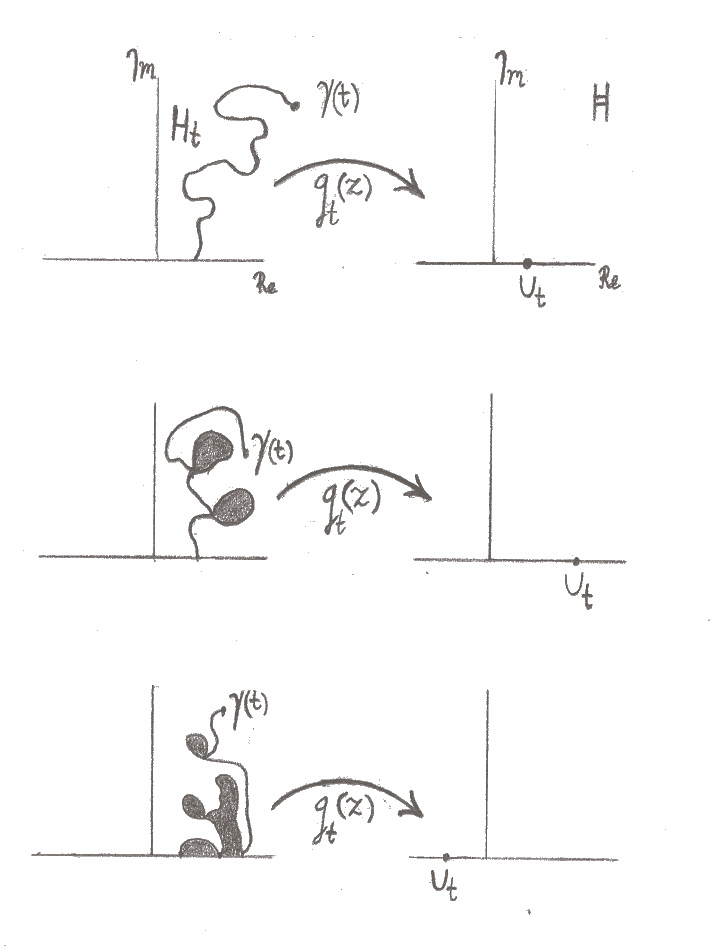
\includegraphics[width=6cm,height=6cm]{firstex.png}
\end{figure}

\end{frame}

\begin{frame}[fragile]
  \frametitle{birds eye}
  % what is the contribution of fshark
  
  %% c# computational kernel generator for futhark
  %%% short explanation of current state of futhark
  %%% use case for futhark c# code generator
  %%% show diagram of futhark compilation pipeline
  %%%% for each part, elaborate and show example

  %% language with library
  %%% explain use case
  %%% show short code example

  %% fshark transpiler and wrapping framework
  %%% explain use case
  %%% show large diagram of components, and explain individual parts
  %%%% for each part, elaborate and show example
  

\begin{figure}
  \centering
 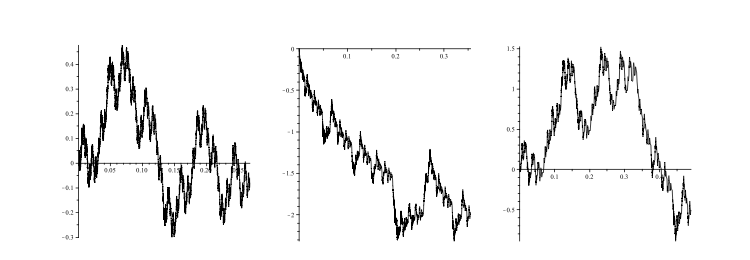
\includegraphics[width=11cm,height=4cm]{intro2.png}
\end{figure}
\tiny
source: "spacefilling curves and phases of the loewner equation", j.lind, s.rohde
\normalsize
\end{frame}

\begin{frame}[fragile]
  \frametitle{Challenging aspects of the implementation}

  
  % Choosing what types FShark should support, and how to implement the support
  % for these types. in particular the whole ding about arrays.


\begin{figure}
  \centering
 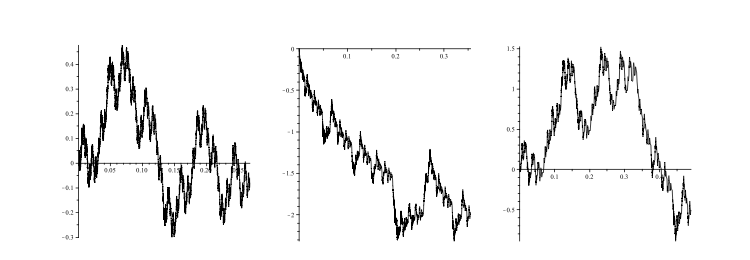
\includegraphics[width=11cm,height=4cm]{intro2.png}
\end{figure}
\tiny
source: "spacefilling curves and phases of the loewner equation", j.lind, s.rohde
\normalsize
\end{frame}

\begin{frame}[fragile]
  \frametitle{Evaluation}

  

\begin{figure}
  \centering
 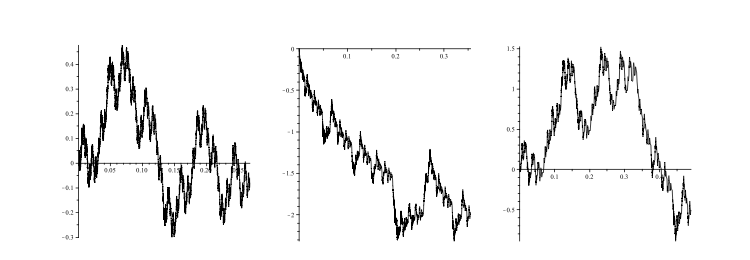
\includegraphics[width=11cm,height=4cm]{intro2.png}
\end{figure}
\tiny
source: "spacefilling curves and phases of the loewner equation", j.lind, s.rohde
\normalsize
\end{frame}

\begin{frame}[fragile]
  \frametitle{Evaluation - Testing and correctness}

  

\begin{figure}
  \centering
 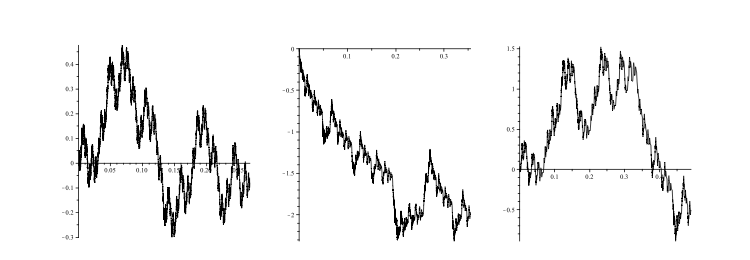
\includegraphics[width=11cm,height=4cm]{intro2.png}
\end{figure}
\tiny
source: "spacefilling curves and phases of the loewner equation", j.lind, s.rohde
\normalsize
\end{frame}


\begin{frame}[fragile]
  \frametitle{Evaluation - Performance}

  

\begin{figure}
  \centering
 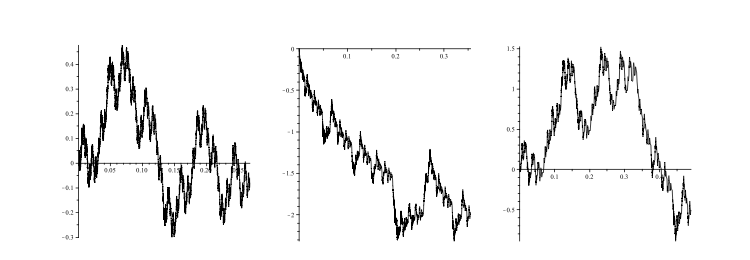
\includegraphics[width=11cm,height=4cm]{intro2.png}
\end{figure}
\tiny
source: "spacefilling curves and phases of the loewner equation", j.lind, s.rohde
\normalsize
\end{frame}

\begin{frame}[fragile]
  \frametitle{Evaluation - Usability and interoperability}

  

\begin{figure}
  \centering
 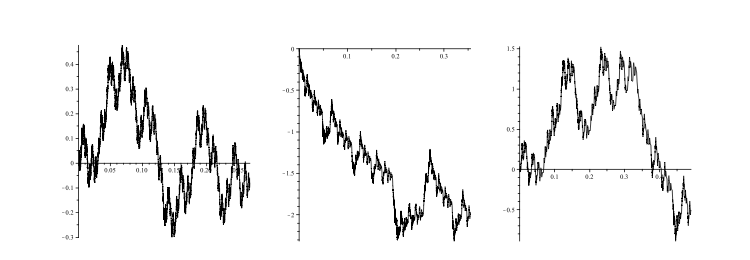
\includegraphics[width=11cm,height=4cm]{intro2.png}
\end{figure}
\tiny
source: "spacefilling curves and phases of the loewner equation", j.lind, s.rohde
\normalsize
\end{frame}


\begin{frame}[fragile]
  \frametitle{Related work}

  

\begin{figure}
  \centering
 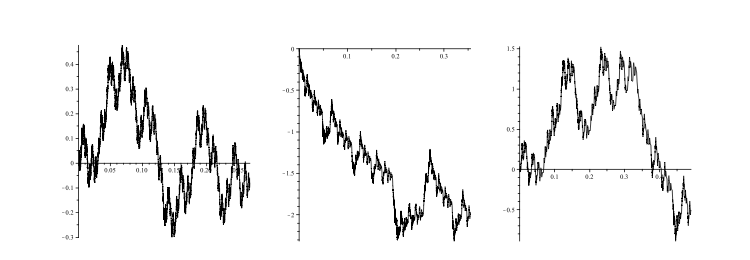
\includegraphics[width=11cm,height=4cm]{intro2.png}
\end{figure}
\tiny
source: "spacefilling curves and phases of the loewner equation", j.lind, s.rohde
\normalsize
\end{frame}






\begin{frame}[fragile]
  \frametitle{Illustrations}
And the sets they generate
\begin{figure}
  \centering
 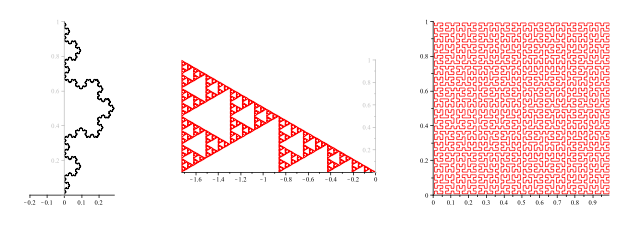
\includegraphics[width=8cm,height=4cm]{intro1.png}
 \caption{van Koch curve, the half-Sierpinski gasket, and the Hilbert space-filling curve}
\end{figure}
\tiny
Source: "Spacefilling Curves and Phases of the Loewner Equation", J.Lind, S.Rohde
\normalsize
\end{frame}

\begin{frame}[fragile]
  \frametitle{the SLE-curve}
Let $U_{t}=\sqrt{\kappa}B_{t}$, where $\kappa \in \mathbb{R}$ and $B_{t}$ is a standard Brownian motion. Then, with probability one, the set $H_{t}$ is generated by a curve, i.e $H_{t}=\mathbb{H}\backslash \gamma(0,t]$ for some continuous curve $\gamma$. This $\gamma$ is called an SLE-curve. Two interesting facts about the SLE-curve:


\begin{itemize}
\item The curve spirals at every point
\item The trace is extremely sensitive to the value of $\kappa$. In fact 
\begin{itemize}
\item For $0 \leq \kappa \leq 4$ the trace $\gamma$ is simple with probability one.
\item For $4 \leq \kappa < 8$ the trace $\gamma$ intersects itself and every point is contained in a loop but the curve is not space-filling (with probability 1).
\item For $\kappa \geq 8$ the trace $\gamma$ is space-filling (with probability 1).
\end{itemize}
\end{itemize}

\end{frame}

\begin{frame}[fragile]
  \frametitle{Illustrations}
$\kappa=2$, yielding a simple trace:
\begin{figure}
  \centering
 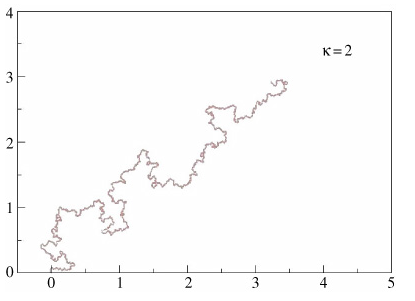
\includegraphics[width=8cm,height=4cm]{simple.png}
\end{figure}
\small
Source: http://iopscience.iop.org
\normalsize
\end{frame}

\begin{frame}[fragile]
  \frametitle{Illustrations}
$\kappa=6$, yielding a non-simple trace:
\begin{figure}
  \centering
 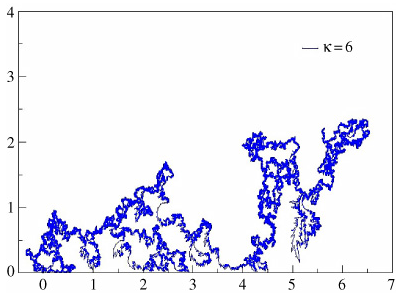
\includegraphics[width=8cm,height=4cm]{nonsimple.png}
\end{figure}
\small
Source: http://iopscience.iop.org
\normalsize
\end{frame}

\begin{frame}[fragile]
  \frametitle{Discrete Gaussian free fields}
Rougher grid left, finer grid right
\begin{figure}
  \centering
 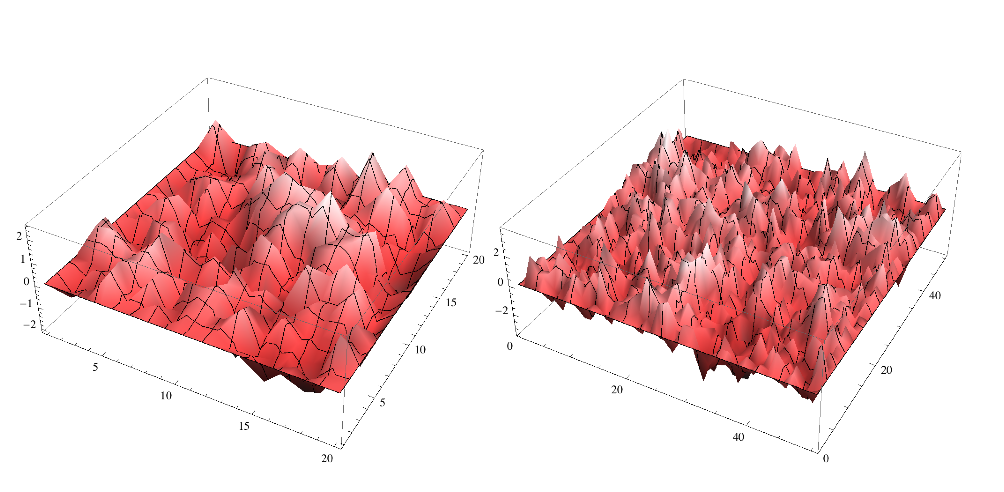
\includegraphics[width=8cm,height=4cm]{gaussian.png}
\end{figure}
\small
Source: "Finding SLE paths in the Gaussian free field ", S.L. Watson
\normalsize
\end{frame}

\begin{frame}[fragile]
  \frametitle{Purpose of Third part}
Aim: Investigate upper bounds of the quantity $|\arg g^{-1 \prime}_{t}(z)|$ as $z$ approaches the boundary, for driving functions of H\"older-1/2 continuous driving functions\\

(Recall H\"older-1/2 continuity: $|U_{t+s}-U_{t}| \leq \sigma \sqrt{s}$ for some $\sigma \in \mathbb{R}^{+}$)


\end{frame}

\begin{frame}[fragile]
  \frametitle{Apriori expectations}
\begin{itemize}
\item $\boldsymbol{\sigma<2\sqrt{2}}$: Nontrivial bound for argument should exist and this should be possible to prove with methods from RTZ\\

\item $\boldsymbol{2\sqrt{2} \leq \sigma < 4}$. Non-trivial bound should exist for the argument since it does exist for the absolute value for $\sigma <4$; but this cannot be proved with methods outlined in RTZ
\end{itemize}
\end{frame}

\begin{frame}[fragile]
  \frametitle{An illuminating example}
  \small
In the article "Collisions and spirals of Loewner traces" by Lind, Marshall and Rohde, the Loewner trace and conformal map of the driving function $U_{t} = \sigma\sqrt{1-t}$, $0 < \sigma < 4$ are calculated. In fact here the following is stated:\\

Given $0 < \sigma < 4$, set $\theta := -\sin^{-1}(\sigma/4)$, $\beta = 2ie^{i\theta}$, and set

\begin{center}
$k(z) = \frac{(z-\beta)(z-\bar{\beta})^{e^{2i\theta}}}{(\sigma - \beta)(\sigma - \bar{\beta})^{e^{2i\theta}}}$ \\
$g_{t}(z) = (1-t)^{1/2}k^{-1}((1-t)^{-\cos\theta e^{i\theta}}k(z))$ 
\end{center}

Then $k$ is a conformal map of $\mathbb{H}$ onto $\mathbb{C}\backslash G$ where $ G := \{e^{te^{i\theta}} ; t \geq 0 \}$, is a logarithmic spiral in $\mathbb{C}$ beginning at $1$ and tending to $\infty$, and where $g_{t}$ satisfies the Loewner equation 
\begin{center}
$\displaystyle{\dot g_{t} = \frac{2}{g_{t} - \sigma\sqrt{1-t}} \; g_{0} \equiv z} $
\end{center}
The trace $\gamma = k^{-1}(\{e^{-te^{i\theta}} ; t > 0\})$ is a curve in $\mathbb{H}$ beginning at $\sigma \in \mathbb{R}$ spiraling around $\beta \in \mathbb{H}$

\normalsize
\end{frame}

\begin{frame}[fragile]
  \frametitle{}
\begin{figure}
 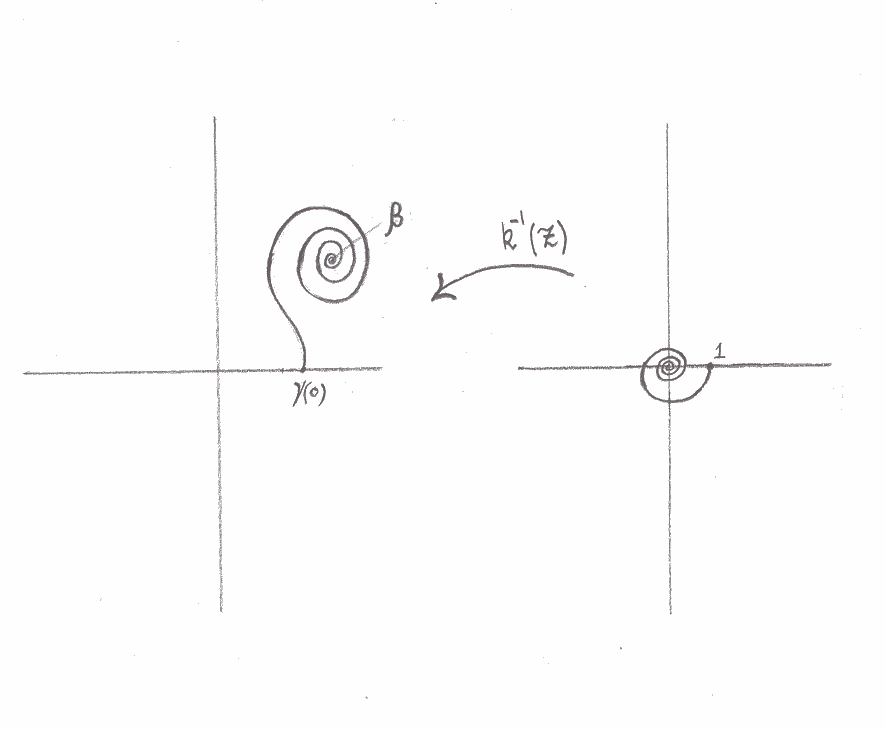
\includegraphics[width=10cm,height=8cm]{spiral.png}
\end{figure}
\end{frame}

\begin{frame}[fragile]
  \frametitle{Results}
\begin{itemize}
\item $\boldsymbol{\sigma<\sqrt{2}}$: A non-trivial bound is obtained in line with expectation. \\

\item $\boldsymbol{\sqrt{2} \leq \sigma < 2\sqrt{2}}$: We show the methods of RTZ are insufficient for obtaining a non-trivial bound in this interval. However, we still suspect such a nontrivial bound to exist\\

\item $\boldsymbol{2\sqrt{2} \leq \sigma < 4}$: We have shown no non-trivial bound can exist in this interval
\end{itemize}
\end{frame}

\plain{Questions?}

\end{document}